\documentclass{article}
\usepackage{float} % this is for image placement
\usepackage{blindtext}
\usepackage{fullpage}
\usepackage{graphicx} % this is so that we can have images
\graphicspath{{/images}} %path to images

\usepackage{biblatex}
\addbibresource{references.bib}

\renewcommand*\contentsname{Table of Contents} % changing the default title of table of contents simply from "contents"


%here we add Abstract and acknowledgement to table of contents despite them being unnumbered sections



\title{Future of Clothing, A technological approach}
\author{Dinesh Devkota,
Maharshi Bhusal, Rajat Parajuli, Sushant Thapa}
\date{\today}


\begin{document}

\pagenumbering{roman}
\begin{figure}[H]
    \centering
    
\includegraphics[width=5cm]{images/tuLogo.png}
\end{figure}

\begin{center}
\textbf {{\Huge Future Of Clothing}}
\end{center}

\begin{center}
\textbf {{\huge A Technological Approach}}
\end{center}

\begin{center}

Submitted To
\end{center}

\begin{center}
\textbf {{\huge The Department Of Electronics and Computer Engineering}}
\end{center}

\begin{center}
\textbf {{\Small Institue of Engineering, Pulchowk Campus}}
\end{center}

\begin{center}

Dinesh Devkota, 073BCT516
\end{center}

\begin{center}
Maharshi Bhusal, 073BCT522
\end{center}

\begin{center}
Rajat Parajuli, 073BCT532
\end{center}

\begin{center}
Sushant Thapa, 073BCT547
\end{center}

\begin{center}

\today
\end{center}
\newpage
    \section*{Acknowledgement}
\addcontentsline{toc}{section}{Abstract} % it is important to add this line after section, instead of before the \begin{document} line as doing so generates erroneous output
We would like to express our gratitude to the Department of Electronics and Computer Engineering of the Institute of Engineering, Pulchowk Campus for providing a platform for exchanging knowledge and developing one’s personal creativity. All guidance and resources provided by the college has been crucial in our vision that we present today. By assigning a major project as part of the fulfilment of the Bachelors’ Degree in Computer Engineering, the Department has helped us develop technical skills and convey the necessities in handling real life projects in the future.
We are indebted to Dr Jyoti Tandukar for being our supervisor and guiding us towards a feasible project roadmap. His guidance, experiences and expertise have been a boon for our group and crucial in developing our project to the stage it has reached. We would also like to extend our gratitude to the staff of Alternative Technology who have supported us throughout our project timeline.



\newpage

\section*{Abstract}
\addcontentsline{toc}{section}{Acknowledgement}
The project “The Future of Clothing: A Technological Approach” is a project that aims to use existing technology to improve the experience of custom designed clothing. Here, a program is written for the design of the clothes and generation of a human body model, both on the basis of user input and preference. The program further wraps the generated clothing on the body model and enables the end-user to view this model in a 3-D environment.
\newpage

\tableofcontents
\listoffigures


\newpage
\pagenumbering{arabic}
\section{Introduction}


Technology in the sector of image processing has matured enough for developers to create interesting applications. With the increase in computation power, software development tools, developer communities, etc. and decrease in the cost of computer hardware it has become easier for technology creators and consumers to create and consume technology for a better quality of life.
In this project, the attention is focused towards using technology in the field of image processing and applying the said technology towards clothing. The main aim of the project is to create a system whereby a user can virtually wrap a computer generated cloth to a computer generated body of the end user. The body of the subject is based on the description provided by the users themselves. Not only is the clothing wrapped around a user defined body wireframe, but the clothing and the pattern of clothing is also user defined providing a high degree of customization from the perspective of the user. 
Patterns and designs used in the clothing can be generated by using a generative adversarial network (GAN) which will synthesize brand new designs and patterns based on the user’s preference. Such a GAN can be trained by supplying training data according to the user preference.
\newpage
\section{Literature Review}
\subsection{Generative Adversarial Networks}

\begin{figure}[H]
    \centering
    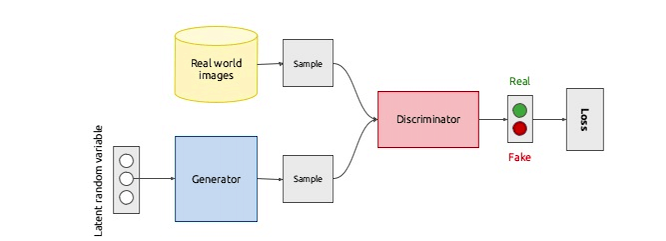
\includegraphics[width=15cm]{images/GAN/basicGAN.png}
    \caption{Basic GAN}
    \label{fig:my_label}
\end{figure}
Generative Adversarial Networks (GANs) are a class of the deep neural networks which works by competing two networks namely Generative and Adversarial networks.This network was defined and introduced to the world by Ian Goodfellow in 2014 in a now legendary paper. Generative Adversarial Network consist of two networks. A generative network and an Adversarial network. The generative network is a simple network which takes in gaussian noise as input and then scales and modifies the noise to create a new generated image. This generated image is the result of the GAN we need. New examples from the GANS are generated on the basis of this noise and the network. The adversarial network on the other hand is generally a classifier based on Convolutional networks. The architecture of the generative and adversarial network is not defined anywhere but generally a modified Convolutional network for adversarial and Transpose Convolutional network for generative network. However the original paper introducing GANs. It was a fully connected network for both generative and adversarial networks.
The Generative and Adversarial network compete in a game to fool one another, sort of like a race. On each epochs,the generative network or generator generates new images based on the input noise  the adversarial network learns from the training data and then uses that information to verify image produced by the generative network. The real image is classified as true for the discriminator while the generated image is classified as false. Now the loss is calculated and is used to update both discriminator and the generator. If all goes well, after a few epochs the generator is able to fool the discriminator with a generated image and we get a very lifelike and real image.
 
Our architecture aims to provide a high quality geometric shapes as output. So vanilla GANs with fully connected networks cannot work as the one required as per our project. Thus we have looked into several other variation of GANs which we hope to mix in our architectures.

\subsubsection{Deep Convolutional GAN}
Deep Convolutinal GAN is a variation of GAN which is based on Deep Convolutional architecture. It uses Deep Convolutinal architecture for the dicriminator as well as Transpose Convolutional to scale the image from the noise in the generator.The paper on DCGAN presents it as a topologically constrained variant of conditional GAN. The main benifit of usig DCGAN over classical GAN is that they are more stable to train and very useful in training unsupervised image representations. Furthermore, GANs are difficult to scale using CNN. The paper proposes to replace pooling layers with strided convolution i.e. no fully connected layers and replace it with convolutional counterparts. it further proposes to use LeakyReLU and batch normalization in all layers of discriminator while using ReLU and batch normalization in all layers of the generator(except output).
\begin{figure}
    \centering
    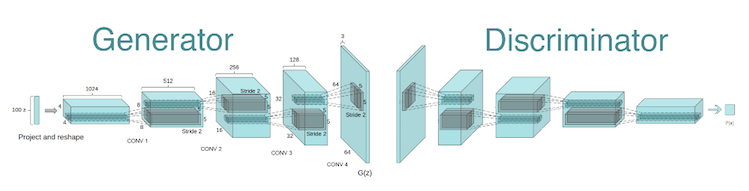
\includegraphics[width=15cm]{images/GAN/DCGAN.png}
    \caption{Caption}
    \label{Architecture of Deep Learning GAN}
\end{figure}

\subsubsection{StackGAN}
A very innate problem of both DCGAN and vanilla GAN is that they are unable to be scaled to higher degree. GAN is structurally an unstable architecture and it needs a lot of work to achieve momentary stability. Furthermore the complexity of any image based neural network increases exponentially with the increase in the size of the input and output. Thus the GANs which consist of large image input and output are very unstable and require a lot of processing power along with other complications in the training method. A new system was proposed to increase the size and quality of the image produced by the GAN. In layman terms this paper proposes to stack the output of smaller GANs to the larger GANs and increase the size of the output in two times increment.

\subsubsection{StyleGAN}
GANs are very successful to provide high quality image of the natural environments and natural structures. However, vanilla and most other types of GAN fail to provide satisfactory output for a more geometric and cartoony images. StyleGAN aims to remove this problem through using a random noise in the middle of a generator architecture which will help with the sharper ends of the images. As per the website, generation of animation faces, which is similar in structure to motifs and designs are difficult to create using simple GAN architecture including the vanilla GAN architecture. The author also moves on to explain that the creation of the faces is faster and more accurate using a variant of GAN called StyleGAN.Style GAN is a Style-Based Generator Architecture for Generative Adversarial Networks is an alternative generator architecture for generative adversarial networks, borrowing from style transfer literature. The new architecture leads to an automatically learned, unsupervised separation of high-level attributes.


\subsubsection{ProGAN}
GANs have always been very hard and large to train. A group of researchers of NVIDIA corporation did extensive research and have proposed a better way to train GANs. Large GANs which have very large output donot seem to scale well with complexity.
\subsubsection{WarrensteinGAN}
GANs are very difficult to train. This difficulty is in part thanks to having no good metric to provide a way to measure the success of the GANs and other generating networks. Thus the researcher are pretty much eyeballing the learning rates and other mechanism of the design. WarrensteinGAN tries to make the learning method more easy by proposing a newer and better metric to calculate the loss of the gan and provide a way to quantify their progress. WarrensteinGAN uses earth distance as a progress bar to measure the advancement of the training and provides pretty good result.

\subsubsection{Least Square GAN}

WGANs proposed to address the problem by using the EMD or Wasserstein loss function which has a smooth differentiable function even when there is little or no overlap between the two distributions. However, WGAN is not concerned with the generated image quality. Apart from stability issues, there are still areas of improvement in terms of perceptive quality in the generated images of the original GAN. LSGAN theorizes that the twin problems can be solved simultaneously.
LSGAN proposes the least squares loss. 

Ideally, the fake samples distribution should be as close as possible to the true samples' distribution. However, for GANs, once the fake samples are already on the correct side of the decision boundary, the gradients vanish.

 Using the least squares loss function, the gradients do not vanish as long as the fake samples distribution is far from the real samples' distribution. The generator will strive to improve its estimate of real density distribution even if the fake samples are already on the correct side of the decision boundary.
   
    \subsection{3D Human Model Construction }
There has been a lot of work done in the construction, use and manipulation of three-dimensional human body models for various purposes. Many researchers have used 3D full body scanners, 3D cameras and even the Xbox Kinect camera to capture and map human models. Similarly, a lot of research has be done to manipulate and generate new human models from the assets available by training regression functions to correlate semantically significant values or by employing the use of principal component analysis on feature curves and segment patches drawn onto the model and thus modified. Our project will employ a mix of principal component analysis and linear regression models to generate parameters on the human body model and allow general modifications.

\subsection {UV Mapping}
UV mapping is the process of mapping textures from an image into the surfaces of a 3D object. We cannot simply attach a 2D image to a 3D object we have to map every surface to a portion of the image. Since we knew where the triangles were taken from in the image, we knew exactly which portion of the image should be mapped to which surface.
There has been a lot of work done in the construction, use and manipulation of three-dimensional human body models for various purposes. Many researchers have used 3D full body scanners, 3D cameras and even the Xbox Kinect camera to capture and map human models. Similarly, a lot of research has be done to manipulate and generate new human models from the assets available by training regression functions to correlate semantically significant values \cite{Exemplar} or by employing the
use of principal component analysis on feature curves and segment patches drawn onto the model
and thus modified \cite{Exemplar}. Our project will employ a mix of principal component analysis and linear
regression models to generate parameters on the human body model and allow general
modifications.
Among the many datasets available, the MPII Human Shape dataset \cite{StatisticalShapeSpaces} \cite{poisson} is a readily available free
dataset that was used which was based on the widely used statistical body representation and
learned from the CAESAR dataset, the largest commercially available scan database to date. The
Polygon File Format (.ply) files obtained from the dataset formed the generic point cloud shape of
the human body which was further processed in a commercially available software MeshLab \cite{meshlab} \cite{poisson} for the calculation of normal and triangulation. Further work could employ Delaunay
triangulation and also spherical parameterization of 3D meshes \cite{sphericalParam} for more optimized mesh
construction, manipulation and also for better texture mapping.


\newpage
\section{Significant Programming Tools, Libraries and Methods}

	\subsection{WebGL and Three.js}

	Three.js uses WebGL to draw 3D. WebGL is a very low-level system that only draws points, lines, and triangles. To do anything useful with WebGL generally requires quite a bit of code and that is where three.js comes in. It handles stuff like scenes, lights, shadows, materials, textures, 3d math, all things that one would have to write yourself if you were to use WebGL directly. \cite{threejsfundamentals} 

	   \begin{figure}[H]
            \centering
            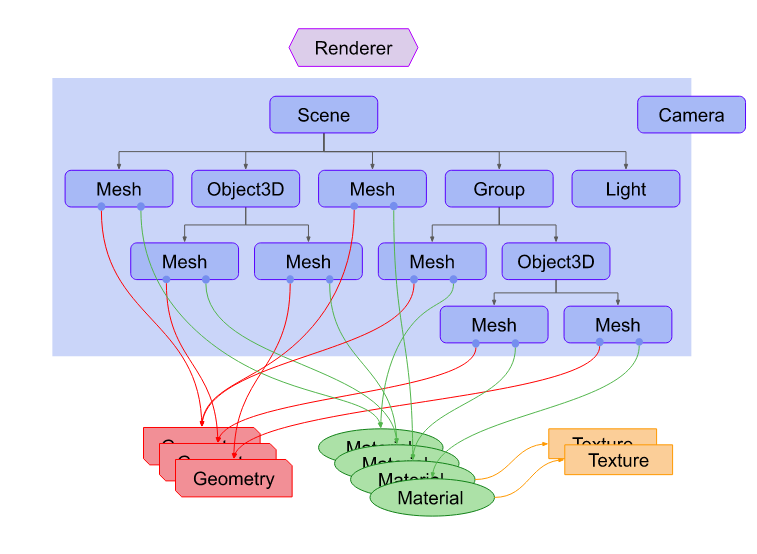
\includegraphics[width=15cm]{images/threeDotJS/threeJsStructure.png}
            \caption{Basic Structure of Three.js}
        \end{figure}
    \subsubsection{Renderer}
    This is one of the main objects of three.js. A scene and a camera is to a Renderer and it renders (draws) the portion of the 3D scene that is inside the frustum of the camera as a 2D image to a canvas.

    \subsubsection{Scene Graph}  A scene graph in a 3D engine is a hierarchy of nodes in a graph where each node represents a local space. It is a tree like structure, consisting of various objects like a Scene object, multiple Mesh objects, Light objects, Group, Object3D, and Camera objects.
    A Scene object defines the root of the scene graph and contains properties like the background color and fog. These objects define a hierarchical parent/child tree like structure and represent where objects appear and how they are oriented. Children are positioned and oriented relative to their parent. 
    \begin{figure}[h]
            \centering
            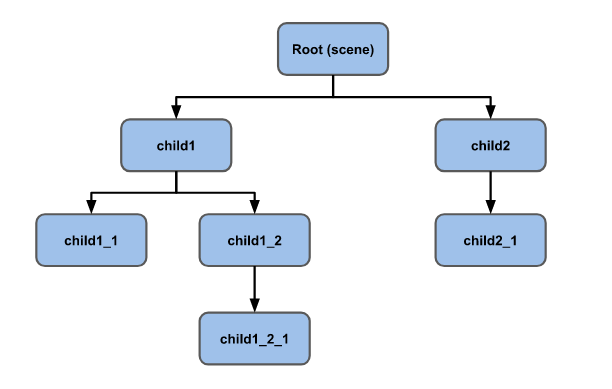
\includegraphics[width=15cm]{images/threeDotJS/sceneGraph.png}
            \caption{Scene Graph Structure}
        \end{figure}
        
    \subsubsection{Camera}
    A camera in three.js is a child of an object, but does not have to be inside the scene graph to function. The most common camera in three.js and the one used in our application is the PerspectiveCamera. It gives a 3d view where things in the distance appear smaller than things up close.

The PerspectiveCamera defines a frustum, which is a solid pyramid shape with the tip cut off.

A PerspectiveCamera defines its frustum based on 4 properties, 
    \begin{enumerate}
    \item \textbf{near} : It defines where the front of the frustum starts.
    \item \textbf{far}: It defines where it ends.
    \item \textbf{fov} : The field of view, defines how tall the front and back of the frustum are by computing the correct height to get the specified field of view at near units from the camera. This is measured in degrees.
    \item \textbf{aspect} : It defines how wide the front and back of the frustum are. The width of the frustum is just the height multiplied by the aspect.
    
    \end{enumerate}
    
    
    \subsubsection{Mesh objects}
    Mesh objects represent drawing a specific Geometry with a specific Material. Both Material objects and Geometry objects can be used by multiple Mesh objects. 
    \paragraph{Geometry objects} represent the vertex data of some piece of geometry like a sphere, cube, plane, dog, cat, human, tree, building and so forth. Three.js provides many kinds of built in geometry primitives. Custom geometry can also be created and geometry can be loaded from files as well.
    
    \paragraph{Material objects} represent the surface properties used to draw geometry including things like the color to use and how shiny it is. A Material can also reference one or more Texture objects which can be used, for example, to wrap an image onto the surface of a geometry.
    
    \subsubsection{Texture objects}
    Texture objects generally represent images either loaded from image files, generated from a canvas or rendered from another scene.

    \subsubsection{Light objects}
    Light objects represent different kinds of lights. Some of the important ones are 
    \begin{enumerate}
        \item {Ambient Light}: This light globally illuminates all objects in the scene equally.This light cannot be used to cast shadows as it does not have a direction.
        \item {Hemisphere light} :A light source positioned directly above the scene, with color fading from the sky color to the ground color.This light cannot be used to cast shadows.
        \item {Directional Light}:  A Directional Light is often used to represent the sun.A light that gets emitted in a specific direction. This light will behave as though it is infinitely far away and the rays produced from it are all parallel. The common use case for this is to simulate daylight. This light can cast shadows.
        \item{Point Light}: A Point Light is a light that sits at a point and shoots light in all directions from that point.  A common use case for this is to replicate the light emitted from a bare lightbulb.This light can cast shadows 
        \item{Spotlight}: Spotlights are effectively a point light with a cone attached where the light only shines inside the cone. There's actually 2 cones. An outer cone and an inner cone. Between the inner cone and the outer cone the light fades from full intensity to zero.This light can cast shadows.
    \end{enumerate}


\section{Methodology}

    \subsection{Basic Structure of System}
        \begin{figure}[h]
            \centering
            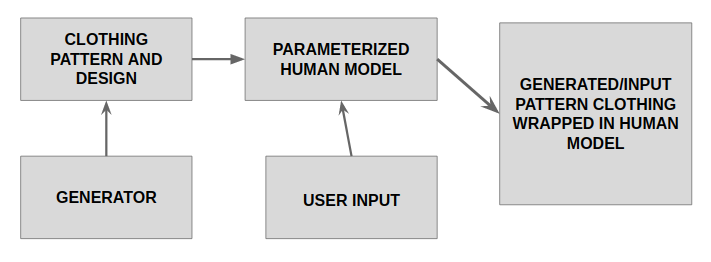
\includegraphics[scale=0.75]{images/basicArchitecture.png}
            \caption{basic architecture of system}
        \end{figure}
    The system is composed of various components, with the major ones shown in figure 2. The generator while generate the patterns which are wrapped in the human model, parameterized by the user input.
    
    \subsection{Image Synthesis using GAN}
    
       On the next step of our experiment we tried to generate a dandelion image from the standard flower dataset which consisted of about 1000 images of dandelion. The kernel from the dog generator was modified and used to fit our new dataset. The new generated image was also 64-by-64 px in size.
    On our next experiment we tried to make a classed generator which takes input a number and outputs the image of different classes on different numbers inputted. The kernel used was a modified version of the TensorFlow tutorial kernel which was taken from a GitHub repository. However, we did not achieve much success with this kernel and thus we used a different architecture which was made by modifying the dog generator kernel.
    The latest experiment involves generation of monochrome motif designs. The motifs are converted to monochrome and then fed to the TensorFlow kernel which did not give us the expected result.
    
    The motif designs were a complex hurdle to complete. The data was few in number and was very high quality which made it very hard to use in the online platform like colab. Furthermore using the data directly to train the network gave very bad results. So, the data needed to be artificially enlarged to give more images. This was done easily using normal data synthesis techniques. A simple proposed pipeline for the GAN training is given below.
    
    \begin{figure}[H]
        \centering
        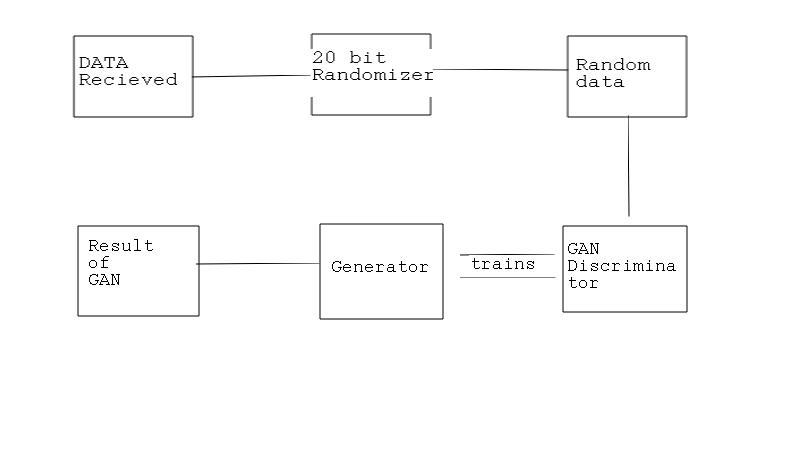
\includegraphics[height=8cm]{images/GAN/Generalworkflow.png}
        \caption{Proposed GAN pipeline}
    \end{figure}
    
    \begin{figure}[H]
        \centering
        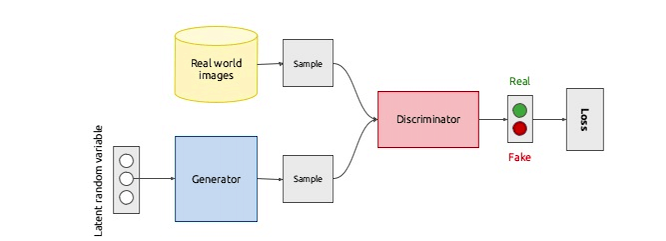
\includegraphics[scale=0.5]{images/GAN/basicGAN.png}
        \caption{Images generated by GAN}
    \end{figure}
    On the next step of our experiment we tried to generate a dandelion image from the standard flower dataset which consisted of about 1000 images of dandelion. The kernel from the dog generator was modified and used to fit our new dataset. The new generated image was also 64-by-64 px in size.
    On our next experiment we tried to make a classed generator which takes input a number and outputs the image of different classes on different numbers inputted. The kernel used was a modified version of the TensorFlow tutorial kernel which was taken from the GitHub repository \textbf{[ CITATION Lam \l 1033 ]}. However, we did not achieve much success with this kernel and thus we used a different architecture which was made by modifying the dog generator kernel.
    The latest experiment involves generation of monochrome motif designs. The motifs are converted to monochrome and then fed to the TensorFlow kernel which did not give us the expected result.
     \subsubsection{Data Acquisition}
    Data acquisition being the first and foremost job in any machine learning project, we also got the data for our experiments early on. Data from various online sources including Kaggle and Google dataset. However we could not find proper and usable data for the motifs and shapes. These data were recieved from alternative technology, which deals with the research in field of ai and image processing.
    The dataset used for Dog and Flower generation were both taken from the Stanford university dataset. These datasets were used to give proper results in the earlier experiments and consisted of about 2000 flowers and 25000 dogs.
    The dataset received from the company was extensive and had about 8000 pictures of varying degrees. Out of those, we used a 300 image rich folder consisting of zigzag lines and blew the size up in the next stage.The data acquired are unclean and mostly consist of 512*512 pixels sized images in png format. The data however seems very varied and may not work in complete perfection. So, the next step will be cleaning the data.
    
    \subsubsection{Data Cleaning}
    There are 77 folders in the data received. The folders were not only populated with images but also consisted of other unwanted files. These unwanted files were scraped and deleted manually. The incoherent directory structure was made coherent by taking the image folders to upper level manually. Most of these folders consist of about >100 images in consistent sizes. These images and folders can be used for image generation. However some consisted of about <30 images. These images can produce noise during training. So, they are kept separately. The incoherent size of images are to be cropped or filled in to provide a coherent size of the image, which will be 512*512 px.
    
    \subsubsection{Synthetic Data Production}
    The remaining data becomes very few in number and it becomes impossible to train the delicately precise GAN with so little data no matter how many epochs it is trained for. So, synthetic data needs to be produced from the present data. Simple procedures are used to make new data from the existing data. The synthetic data production uses four basic transformations for changing data. A basic 6 bit random binary number was generated and used to provide the switch for the application of different transformations. The total variation becomes about 23-bits variations which is quite good considering the limitations of the data. We however use only about 200 samples to increase our data. For a geometric model data like ours, this becomes quite good and gives us very good result.
    They are as follows:
    \begin{itemize}
	\item Stretching and Squashing
	
	The image was stretched and/or squashed by a random pixels from 0 to 15\% of the total size of the image in a step of 3. for a 512 px image it provides 25 different random conditions.
	\item Cropping
	
	The image was cropped upto 10\% of the total width of the image randomly in step of 1. This Gives us about 50 different random conditions in each side, totalling to 100 conditions.
	\item Transpose
	
	Transpose is possible in two ways, horizontal and vertical. Horizontal transpose flips the image horizontally, while vertical transpose flips image vertically.
	\item Rotate
	
	The image can be rotated whole 360 degrees without losing details. Thus we rotate image from 0 to 90 degrees in a step of 1 degree. Thus we have 360 different random conditions for the data
    \end{itemize}
    
    \subsubsection{GAN Training}
    The GAN is then trained to provide new styles. Up until now we have trained the GAN in 28 px square images. However, this will be improved using the stack GAN which will help us with higher size images GAN training. The training took about 11 second per cycle for 28*28 px images which numbered about 56000 in size of the dataset. This GAN was trained for 50 epochs but the best result was seen in the 40th epoch, which was thus used as the final result. Further on the road we aim to get 512*512 size of image using stack GAN. Higher order GANs require a lot more time to train and thus are quite lengthy to train.
    \subsection{Generation of Human Body}
    
    \begin{figure}[h]
        \centering
        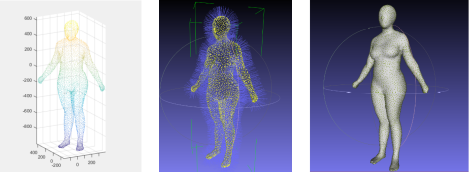
\includegraphics[width=15cm]{images/humanModel.png}
        \caption{(Left) the extracted point cloud. (Middle) The calculated point normal in MeshLab. (Right) The mesh resulting from the screened Poisson surface reconstruction}
        \label{(Left) the extracted point cloud. (Middle) The calculated point normal in MeshLab. (Right) The mesh resulting from the screened Poisson surface reconstruction(Left) the extracted point cloud. (Middle) The calculated point normal in MeshLab. (Right) The mesh resulting from the screened Poisson surface reconstruction}
    \end{figure}
    From the MPII Human Shape dataset, the collection of 4308 models were converted from a .mat format (binary data containers that are used to include variables, functions, arrays, and other information) which contained a 6449x3 matrix of vertices in three-dimensional Cartesian coordinates into a .ply standard polygonal format for the representation of point clouds. These point clouds contained only the basic positional information of the vertices that defined the human body shape. The generated .ply files were imported into a commercially available tool called MeshLab where the point normals were generated. Then the surface was constructed using Screened Poisson Surface Construction method, both of which are available tools in the program. The model was then exported as a Wavefront object (.obj) and ready for further editing.
    
  
    
    
\subsection{Displaying Models}

\begin{figure}[H]
    \centering
    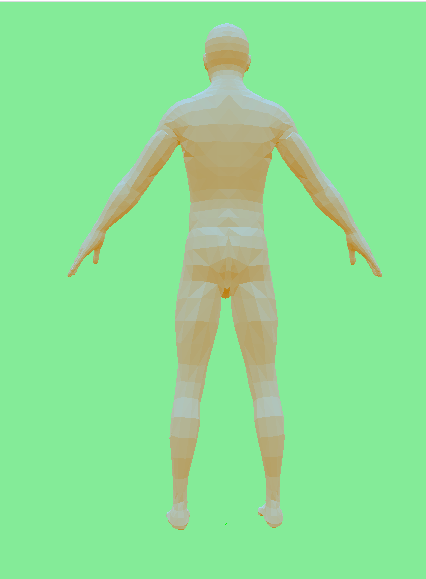
\includegraphics[width=8cm]{images/renderedHumanModel.png}
    \caption{Human Model rendered in the webapp}
    \label{fig:my_label}
\end{figure}

The human model is stored as a wavefront object (.obj), which is loaded via one of the functions provided by three.js. The model is lit by a hemisphere light with a sky color value of 0xB1E1FF(light blue), a ground color of 0xB97A20 (brownish orange) and an intensity of 1. The model was viewed by a Perspective Camera.
\newpage    
\section{Output}

\subsection{GAN outputs}

We have until now trained different and modified versions of opensource, available and stable variation of GANs.Out of different types of GANs these four stand out the most. The type of GANs we have trained includes vanilla GAN with modified structure and DCGAN with pure structure. The vanilla GAN used trained the discriminator first and Generator last to stabilise the training of the GAN. While this provides low quality but stable output, it suffers greatly from mode collapse and dynamic training i.e. training discriminator and generator different times and stopping prematurely. The Vanilla GAN being stable was trained on 64*64 images while the DCGAN was trained on 28*28 images since the GAN was unstable and needed quick experimentation. Previous efforts to port DCGAN was unsuccessful due to the architectural inadequacy. We now however can attempt to do that again with greater chance of success.

\subsubsection{Shapes with Vanilla GAN with Local Dataset}
In this we trained the same GAN structure with about 500 images of floral designs. However, we were unable to get any result due to inherent limitation of the vanilla GAN. From this, we shifted our focus from simple vanilla GAN to advanced variations of GANs, which includes DCGAN and other GANs. The image shown here were trained here with vanilla GAN at 64*64 pixels.
\begin{figure}[H]
    \centering
    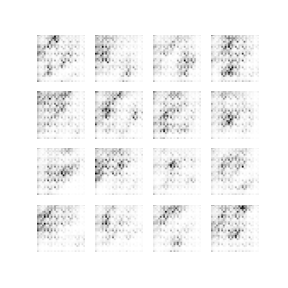
\includegraphics[width=8cm]{images/GAN/GANunmodified.png}
    \caption{Vanilla GAN with Local Unmodified data}
\end{figure}


\subsubsection{ZigZag line with DCGAN with local and synthesized dataset}
In this experiment we conducted two different scenarios. We were trying to experiment with overtraining the GAN with few data on one hand, while we were trying out the synthesized dataset variation on the other hand. The first scenario was however not successful as it didnt produce anything remotely like the dataset provided, no matter how hard we tried. The synthetic dataset however shows promise for the future. The results are shown below.
\begin{figure}[H]
    \centering
    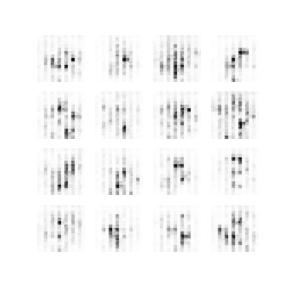
\includegraphics[width=8cm]{images/GAN/DCGANunmodified.png}
    \caption{DCGAN result with Local Unmodified data}
\end{figure}

\begin{figure}[H]
    \centering
    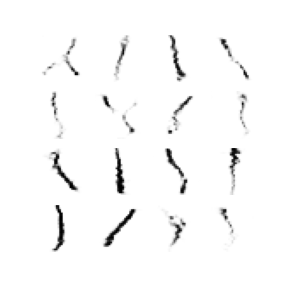
\includegraphics[width=8cm]{images/GAN/DCGANmodified.png}
    \caption{DCGAN result with Synthetic data}
\end{figure}

\section{Software Diagrams}

As stated eloquently in his famous paper, \cite{Brooks87nosilver} Fred Brooks argues software is very difficult to visualize.

He goes on to say " Whether we diagram control flow, variable scope nesting, variable cross-references, data blow, hierarchical data structures, or whatever, we feel only one dimension of the intricately interlocked software elephant. If we superimpose all the diagrams generated by the many relevant views, it is difficult to extract any global overview."

Although it is true that superimposition of various graphical description of the system software does not equate to a whole description of the software, such diagrams can be useful to understand certain aspects of the system and such diagrams are included here.

\begin{figure}[H]
    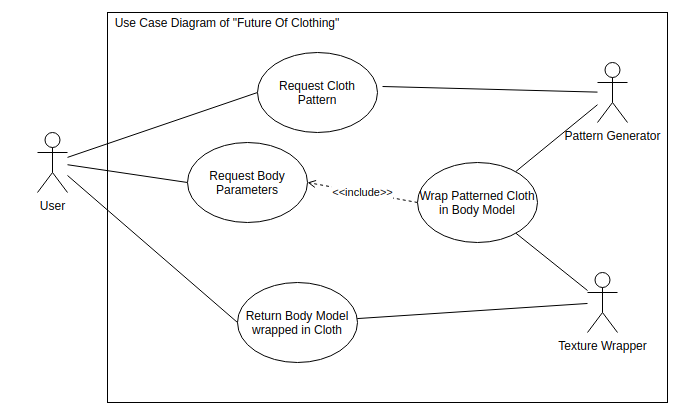
\includegraphics[scale=0.6]{images/softwareDiagrams/FinalSystemUseCase.png}
    \centering
    \caption{Use Case Diagram of the system}
\end{figure}
\paragraph{Use Case} : The use case diagram shows how the user interacts overall with the system and what external entitites are present. The generator and wrapper are shown as part of the system, although being actors.

\begin{figure}[H]
    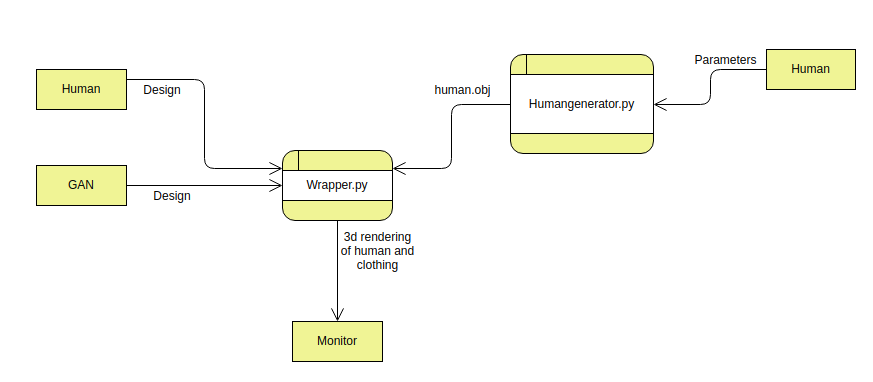
\includegraphics[scale=0.5]{images/softwareDiagrams/DFD.png}
    \caption{Data Flow Diagram of the system}
\end{figure}

\paragraph{Data Flow Diagram}: A Data Flow Diagram, like its namesake, shows how data flows in the system. 
\section{Performance and Analysis}



\section{Conclusion}
\printbibliography
\end{document}